% The Skew-Normal Distribution
\frame{ \frametitle{The Skew-Normal Distribution: Foundations}
  \begin{definition}[Skew-normal]
    Let $Y$ be a skew-normal distribution, with location parameter $\mu \in
    \R$, scale parameter $\sigma > 0$, and shape parameter $\lambda \in \R$.
    Then $Y$ has pdf

    \begin{equation*}
      f(x|\mu, \sigma, \lambda) = \frac2\sigma \cdot \phi \left( \frac{x-\mu}{\sigma} \right) \cdot \Phi \left( \frac{\lambda(x-\mu)}{\sigma} \right), \quad x \in \R,
    \end{equation*}

    where $\phi$ is the standard normal pdf and $\Phi$ is the standard normal
    cdf.

    \vsep
    We write $Y \sim SN(\mu, \sigma, \lambda)$.
  \end{definition}
}
\frame{ \frametitle{The Skew-Normal Distribution: Foundations}
  \tikzstyle{na} = [baseline=-.5ex]

  So where did this funny-looking pdf come from? ...
  \pause
  \begin{lem*}
    If $f_0$ is a one-dimensional probability density function symmetric about
    0, and $G$ is a one-dimensional distribution function such that $G'$ exists
    and is a density symmetric about 0, then
    % Below we mix an ordinary equation with TikZ nodes. Note that we have to
    % adjust the baseline of the nodes to get proper alignment with the rest of
    % the equation.
    \begin{equation*}
      f(z) = 2 \; \cdot
            \tikz[baseline]{
                \node[fill=blue!20,anchor=base] (t1)
                {$f_0(z)$};
            } \cdot
            \tikz[baseline]{
                \node[fill=red!20,ellipse,anchor=base] (t2)
                {$G\{w(z)\}$};
            }
      \quad (-\infty < z < \infty)
    \end{equation*}
    is a density function for any odd function $w(\cdot)$. (Lemma 1,
    \citealp{azzalini})
  \end{lem*}
  \begin{itemize}
    \uncover<3->{
      \item Kernel
        \tikz[na] \node[coordinate] (n1) {};
    }
    \uncover<4->{
      \item CDF
        \tikz[na] \node[coordinate] (n2) {};
    }
  \end{itemize}

  % Now it's time to draw some edges between the global nodes. Note that we
  % have to apply the 'overlay' style.
  \begin{tikzpicture}[overlay]
    \path[->]<3-> (n1) edge [bend right] (t1);
    \path[->]<4-> (n2) edge [bend right] (t2);
  \end{tikzpicture}
}
\frame{ \frametitle{The Skew-Normal Distribution: Foundations}

  Basic properties:

  \begin{align*}
    E(Y) &= \mu + b \delta \sigma \\
    E(Y^2) &= \mu^2 + 2b \delta \mu \sigma + \sigma^2 \\
    E(Y^3) &= \mu^3 + 3 b \delta \mu^2 \sigma + 3 \mu \sigma^2 + 3 b \delta \sigma^3 - b \delta^3 \sigma^3 \\
    Var(Y) &= \sigma^2 (1 - b^2 \delta^2)
  \end{align*}

  where $b = \sqrt{\frac{2}{\pi}}$ and $\delta = \frac{\lambda}{\sqrt{1 +
  \lambda^2}}$. \citep{pewsey}
}
\frame{ \frametitle{The Skew-Normal Distribution: Foundations}

  What happens when $\lambda=0$?
  \pause
  \begin{align*}
    \uncover<+->{f(x|\mu, \sigma, \lambda=0) &= \frac2\sigma \cdot \phi \left( \frac{x-\mu}{\sigma} \right) \cdot \Phi(0) \\}
    \uncover<+->{&= \frac2\sigma \cdot \phi \left( \frac{x-\mu}{\sigma} \right) \cdot 0.5 \\}
    \uncover<+->{&= \frac1\sigma \cdot \phi \left( \frac{x-\mu}{\sigma} \right) \\}
    \uncover<+->{&= \frac{1}{\sqrt{2\pi}\sigma} \;\cdot\; \exp \left( -\frac{(x-\mu)^2}{2\sigma^2} \right),}
  \end{align*}
  \uncover<+->{which is the pdf of the normal distribution ($\mu$, $\sigma$).}
}
\frame{ \frametitle{The Skew-Normal Distribution: The Standard Skew-Normal}

  \begin{definition}[Standard skew-normal]
    The $SN(0,1,\lambda)$ distribution is called the standard skew-normal and
    has pdf

    \begin{equation*}
      f_Z(x|\lambda) = 2 \cdot \phi(x) \cdot \Phi (\lambda x), \quad x \in \R.
    \end{equation*}
  \end{definition}
  \pause

  Similar to the normal and standard normal, $Z = \frac{Y - \mu}{\sigma}$ and $Y
  = \sigma Z + \mu$.
}
\frame{ \frametitle{The Skew-Normal Distribution: The Standard Skew-Normal}
  \begin{property}[1]
    If $Z \sim SN(0, 1, \lambda)$, then $(-Z) \sim SN(0, 1, -\lambda)$.
  \end{property}
  \pause
  \begin{pf}
    \pause
    \begin{align*}
      \uncover<+->{f_{(-Z)}(x) &= f_Z(-x) \\}
      \uncover<+->{& = 2 \cdot \phi(-x) \cdot \Phi (-\lambda x) \\}
      \uncover<+->{& = 2 \cdot \phi(x) \cdot \Phi (-\lambda x),}
    \end{align*}
    \uncover<+->{which is the pdf of $SN(0, 1, -\lambda)$.}
  \end{pf}
}
\frame{ \frametitle{The Skew-Normal Distribution: The Standard Skew-Normal}
  \textit{Property 1}:\; $-SN(0, 1, \lambda) \sim SN(0, 1, -\lambda)$

  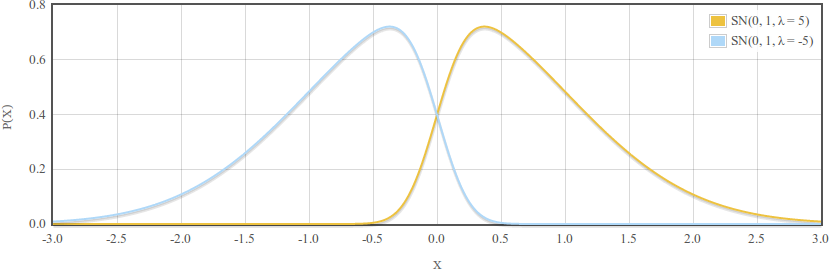
\includegraphics[width=\textwidth]{../images/std-sn-reflection.png}
}
\frame{ \frametitle{The Skew-Normal Distribution: The Standard Skew-Normal}
  \begin{property}[2]
    If $Z \sim SN(0, 1, \lambda)$, then $Z^2 \sim \chi^2_1$ (chi-square with 1 degree of freedom).
  \end{property}
  \pause
  \begin{pf}
    \pause
    Lemma 1 comes with a handy result, (\citealp{azzalini}, page 161):

    If $Y \sim f_0$ and $Z \sim f$, then $|Y| \overset{d}{=} |Z|$, where the
    notation $\overset{d}{=}$ denotes equality in distribution.

    \pause
    Let $X \sim N(0,1)$. Since $X^2 \sim \chi^2_1$ and $|X| \overset{d}{=}
    |Z|$, then $Z^2 \sim \chi^2_1$.
  \end{pf}
}
\frame{ \frametitle{The Skew-Normal Distribution: The Standard Skew-Normal}
  \begin{property}[3]
    As $\lambda \to \pm \infty$, \thinspace $SN(0,1,\lambda)$ tends to the half normal distribution, $\pm |N(0,1)|$.
  \end{property}
  \pause
    Let $X \sim |N(0, 1)|$. Then
    \begin{equation*}
      f_X(x) =
      \begin{dcases*}
        0      & when $-\infty < x \leq 0$ \\
        2 \phi & when $0 < x < \infty$ 
      \end{dcases*}
      .
    \end{equation*}
}
% For some reason, I was obliged to split the following slide into 3 slides, to prevent bumping in between the images.
\frame{ \frametitle{The Skew-Normal Distribution: The Standard Skew-Normal}
  \textit{Property 3}: $SN(0, 1, \lambda) \rightarrow +|N(0,1)|$ as $\lambda \rightarrow \infty$:

  \only<1>{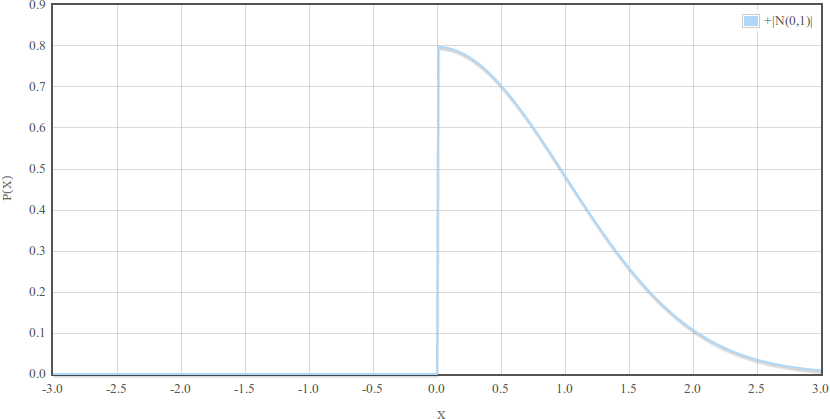
\includegraphics[width=\textwidth]{../images/positive-half-normal.png}}
}
\frame{ \frametitle{The Skew-Normal Distribution: The Standard Skew-Normal}
  \textit{Property 3}: $SN(0, 1, \lambda) \rightarrow +|N(0,1)|$ as $\lambda \rightarrow \infty$:

  \only<1>{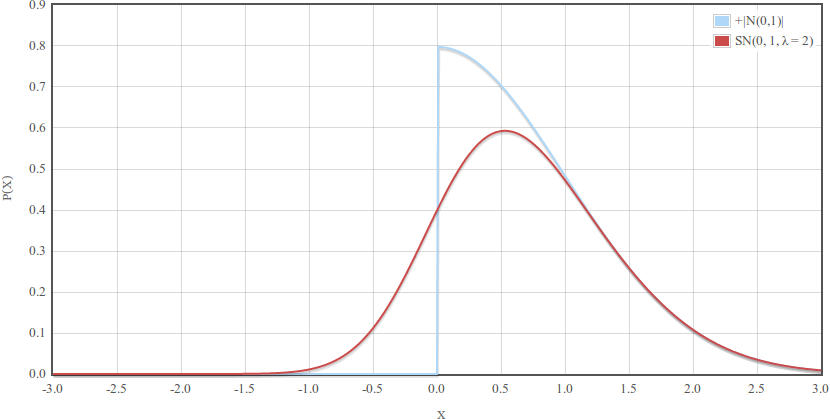
\includegraphics[width=\textwidth]{../images/std-sn-skew2.png}}
  \only<2>{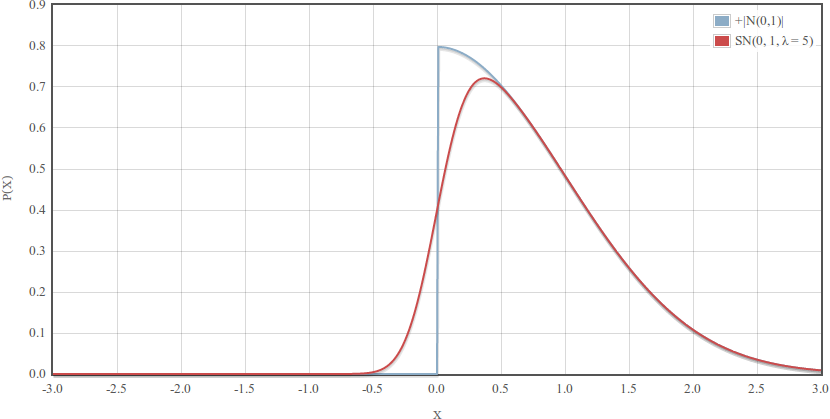
\includegraphics[width=\textwidth]{../images/std-sn-skew5.png}}
}
\frame{ \frametitle{The Skew-Normal Distribution: The Standard Skew-Normal}
  \textit{Property 3}: $SN(0, 1, \lambda) \rightarrow +|N(0,1)|$ as $\lambda \rightarrow \infty$:

  \only<1>{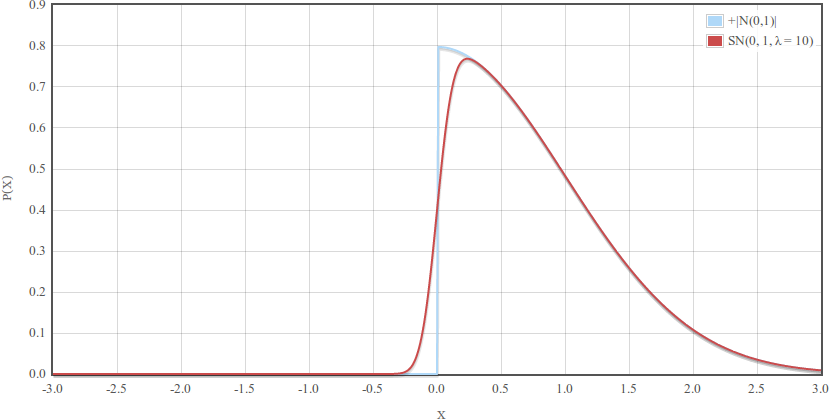
\includegraphics[width=\textwidth]{../images/std-sn-skew10.png}}
  \only<2>{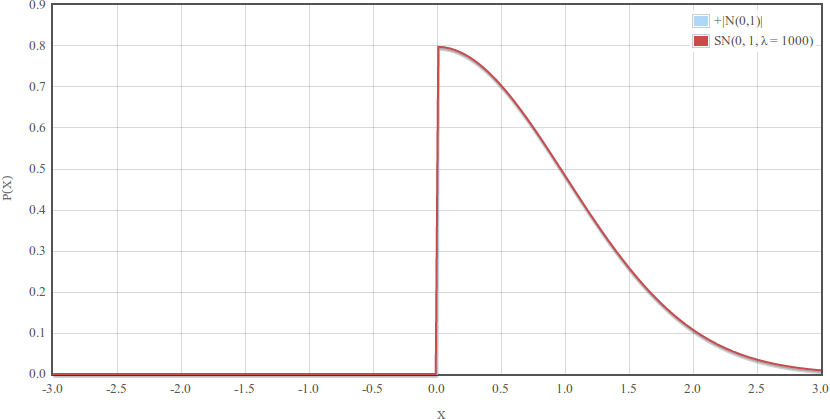
\includegraphics[width=\textwidth]{../images/std-sn-skew1000.png}}
}
% end
% Same bumping issue for this slide
\frame{ \frametitle{The Skew-Normal Distribution: The Standard Skew-Normal}
  \textit{Property 3}: $SN(0, 1, \lambda) \rightarrow -|N(0,1)|$ as $\lambda \rightarrow -\infty$:

  \only<1>{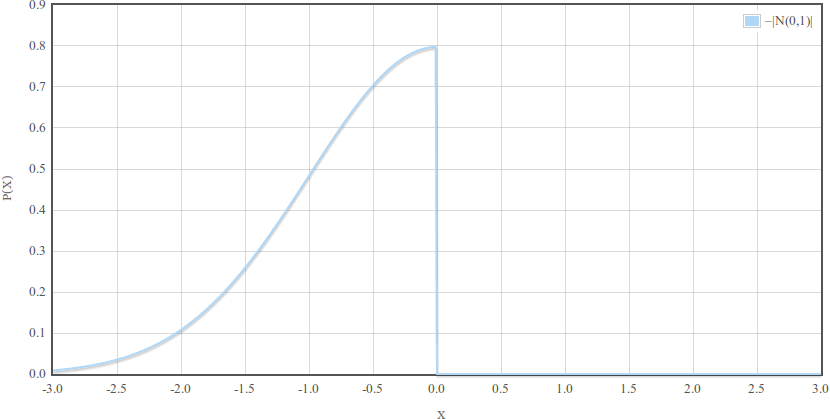
\includegraphics[width=\textwidth]{../images/negative-half-normal.png}}
}
\frame{ \frametitle{The Skew-Normal Distribution: The Standard Skew-Normal}
  \textit{Property 3}: $SN(0, 1, \lambda) \rightarrow -|N(0,1)|$ as $\lambda \rightarrow -\infty$:

  \only<1>{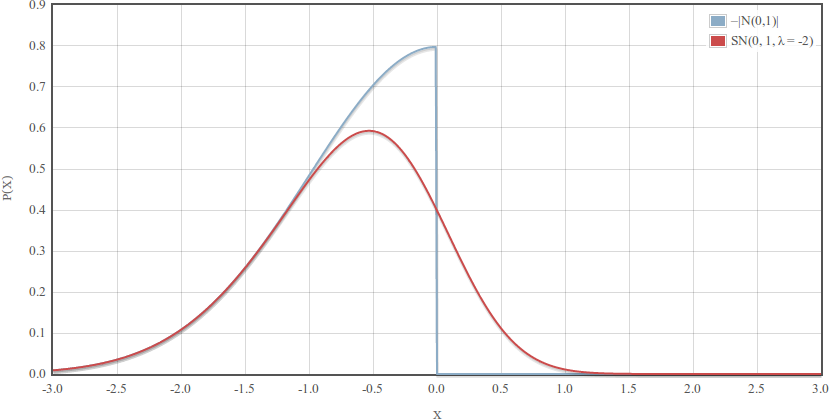
\includegraphics[width=\textwidth]{../images/std-sn-skewneg2.png}}
  \only<2>{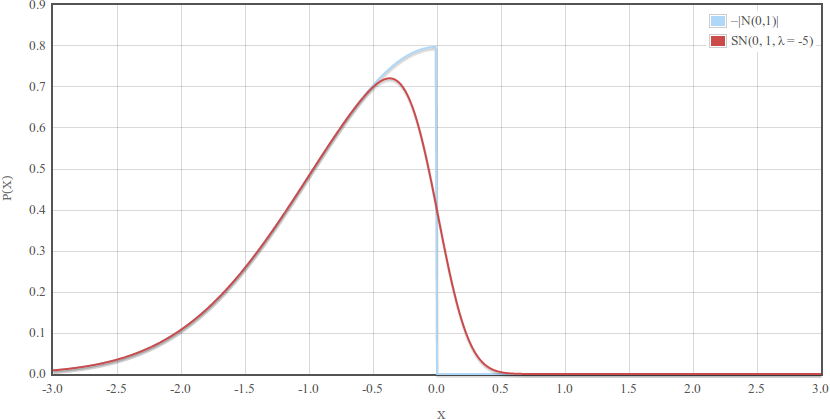
\includegraphics[width=\textwidth]{../images/std-sn-skewneg5.png}}
}
\frame{ \frametitle{The Skew-Normal Distribution: The Standard Skew-Normal}
  \textit{Property 3}: $SN(0, 1, \lambda) \rightarrow -|N(0,1)|$ as $\lambda \rightarrow -\infty$:

  \only<1>{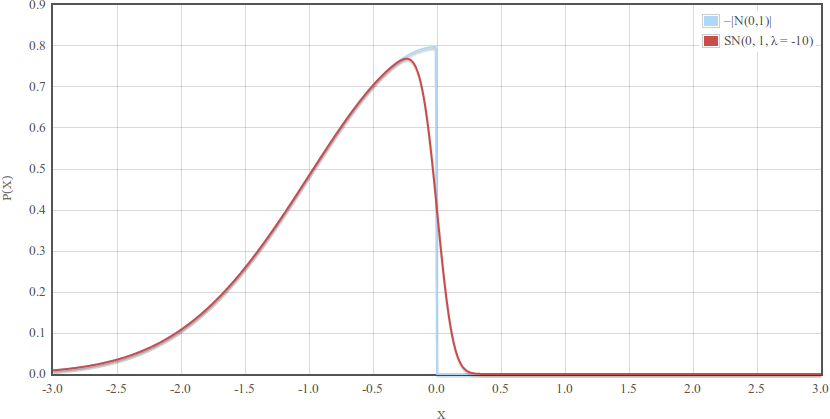
\includegraphics[width=\textwidth]{../images/std-sn-skewneg10.png}}
  \only<2>{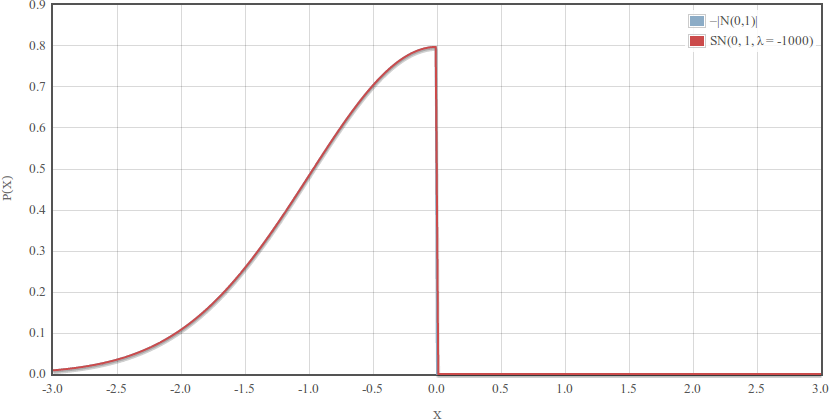
\includegraphics[width=\textwidth]{../images/std-sn-skewneg1000.png}}
}
% end
\frame{ \frametitle{The Skew-Normal Distribution: The Standard Skew-Normal}
  \begin{property}[4]
    The moment generating function of $SN(0,1,\lambda)$ is
    \begin{equation*}
      M(t|\lambda) = 2 \cdot \Phi (\delta t) \cdot e^{t^2/2},
    \end{equation*}
    where $\delta = \frac{\lambda}{\sqrt{1 + \lambda^2}}$ and $t \in (-\infty, \infty)$.
  \end{property}
  \pause
  According to Equation 5 in \citet{azzalini}, the mgf of $SN(\mu, \sigma, \lambda)$ is
  \begin{equation*}
    M(t) \eq E\{e^{tY}\} \eq 2 \cdot \exp \left( \mu t + \frac{\sigma^2 t^2}{2} \right) \cdot \Phi(\delta \sigma t).
  \end{equation*}
  Our result follows.
}
